\documentclass[12pt,pdflatex]{elsarticle} 

%%%%%%%%%%%%%%%%%%%%%%%%%%%%%%%%%%%%%%%%%%%%%%%%%%
%%%%%%%%%%%%%%%%%%%% PREAMBLE %%%%%%%%%%%%%%%%%%%%
%%%%%%%%%%%%%%%%%%%%%%%%%%%%%%%%%%%%%%%%%%%%%%%%%%


% -------------------- defaults -------------------- %
% load lots o' packages

% references
\usepackage{natbib}

% Fonts
\usepackage[default,osfigures,scale=0.95]{opensans}
\usepackage[T1]{fontenc}
\usepackage{ae}
% to colorize links in document. See color specification below
\usepackage[pdftex,hyperref,x11names]{xcolor}
% load the hyper-references package and set document info
\usepackage[pdftex]{hyperref}

% Generate some fake text
\usepackage{blindtext}

% layout control
\usepackage{geometry}
\geometry{verbose,tmargin=1.25in,bmargin=1.25in,lmargin=1.1in,rmargin=1.1in}
\usepackage{parallel}
\usepackage{parcolumns}
\usepackage{fancyhdr}

% math typesetting
\usepackage{array}
\usepackage{amsmath}
\usepackage{amssymb}
\usepackage{amsfonts}
\usepackage{relsize}
\usepackage{mathtools}
\usepackage{bm}
\usepackage[%
decimalsymbol=.,
digitsep=fullstop
]{siunitx}

% restricts float objects to be inserted before end of section
% creates float barriers
\usepackage[section]{placeins}

% tables
\usepackage{tabularx}
\usepackage{booktabs}
\usepackage{multicol}
\usepackage{multirow}
\usepackage{longtable}

% to adapt caption style
\usepackage[font={small},labelfont=bf]{caption}

% footnotes at bottom
\usepackage[bottom]{footmisc}

% to change enumeration symbols begin{enumerate}[(a)]
\usepackage{enumerate}

% to make enumerations and itemizations within paragraphs or
% lines. f.i. begin{inparaenum} for (a) is (b) and (c)
\usepackage{paralist}

% graphics stuff
\usepackage{subfig}
\usepackage{graphicx}
\usepackage[space]{grffile} % allows us to specify directories that have spaces
\usepackage{placeins} % prevents floats from moving past a \FloatBarrier
\usepackage{tikz}
\usepackage{rotating}

% Spacing
\usepackage[singlespacing]{setspace}

% -------------------------------------------------- %


% -------------------- page template -------------------- %

\setlength{\headheight}{15pt}
\setlength{\headsep}{20pt}
\pagestyle{fancyplain}
 
\fancyhf{}
 
\lhead{\fancyplain{}{}}
\chead{\fancyplain{}{Amen for LFM}}
\rhead{\fancyplain{}{\today}}
\rfoot{\fancyplain{}{\thepage}}

% ----------------------------------------------- %


% -------------------- customizations -------------------- %

% easy commands for number propers
\newcommand{\first}{$1^{\text{st}}$}
\newcommand{\second}{$2^{\text{nd}}$}
\newcommand{\third}{$3^{\text{rd}}$}
\newcommand{\nth}[1]{${#1}^{\text{th}}$}

% easy command for boldface math symbols
\newcommand{\mbs}[1]{\boldsymbol{#1}}

% command for R package font
\newcommand{\pkg}[1]{{\fontseries{b}\selectfont #1}}

% approx iid
\newcommand\simiid{\stackrel{\mathclap{\normalfont\mbox{\tiny{iid}}}}{\sim}}

% -------------------------------------------------------- %

%%%%%%%%%%%%%%%%%%%%%%%%%%%%%%%%%%%%%%%%%%%%%%%%%%
%%%%%%%%%%%%%%%%%%%% DOCUMENT %%%%%%%%%%%%%%%%%%%%
%%%%%%%%%%%%%%%%%%%%%%%%%%%%%%%%%%%%%%%%%%%%%%%%%%

% remove silly elsevier preprint note
\makeatletter
\def\ps@pprintTitle{%
 \let\@oddhead\@empty
 \let\@evenhead\@empty
 \def\@oddfoot{}%
 \let\@evenfoot\@oddfoot}

\def\input@path{{/Users/janus829/Dropbox/Research/netModels/summResults/}, {/Users/s7m/Dropbox/Research/netModels/summResults/}, {/Users/mdw/Dropbox/netModels/summResults/}}
\graphicspath{{/Users/janus829/Dropbox/Research/netModels/summResults/}, {/Users/s7m/Dropbox/Research/netModels/summResults/},{/Users/mdw/Dropbox/netModels/summResults/}}
\makeatother

\begin{document}

% saying hello ----------------------------------------------- %
\thispagestyle{empty}
\begin{frontmatter}

\title{Inferential Approaches for Network Analysis: \\ AMEN for Latent Factor Models\tnoteref{t1}}

\tnotetext[t1]{This research was partially supported by the National Science Foundation Award 1259266.}

\author[duke]{Shahryar Minhas\corref{cor1}}
\ead{shahryar.minhas@duke.edu}
\cortext[cor1]{Corresponding author}
\author[duke2]{Peter D. Hoff}
\author[duke]{Michael D. Ward}

\address[duke]{Department of Political Science, Duke University, Durham, NC 27701, USA}
\address[duke2]{Departments of Statistics, Duke University, Durham, NC 27701, USA}

\begin{abstract}
There has been growing interest in the study of political networks. Network analysis allows scholars to focus away from the individual observation toward the interrelationships among observations. This has been particularly strong in the field of international relations, but also has a long tradition in American and Comparative politics as well.  Many network approaches developed in descriptive fashion, and until recently most network studies have been descriptive. Inferential work with networks has been growing.   \citet{cranmer:etal:2016} surveys three, inferential approaches, including the latent space and exponential random graph models of network dependencies.  We present a new approach which presents additive and multiplicative specifications that capture 1st, 2nd, and 3rd order dependencies in network data, whether those data are binary, ordinal, or continuous. In addition this approach, called AMEN,  also allows the incorporation of temporal dependencies.  We develop this approach and compare it to those examined in the survey by Cranmer et alia (2016).  The AMEN approach is shown to be a) easy to implement, b) interpretable in a general linear model framework, c) not faced with computational difficulties, d) avoids the risk of degeneracy in network sampling, e) captures 1st, 2nd, and 3rd order network dependencies, and f) substantially outperforms pseudo-likelihood, multiple regression quadratic assignment procedures, exponential random graph models, and euclidean latent space inferential framework for networks. As such AMEN offers a straightforward way to undertake nuanced, and principled network analysis for a wide range of social science questions involving binary, categorical, and continuous data. 

245 words.
\end{abstract}

\end{frontmatter}
% ----------------------------------------------- %

\newpage\setcounter{page}{1} 

Network analysis provides a way to represent and study ``relational data'', that is data with characteristics extending beyond those of the individual, or in the parlance of International Relations (IR), characteristics beyond the monadic level. Data structures that extend beyond the monadic level are quite simply the norm when it comes to the study of events such as trade, interstate conflict, or the formation of international agreements. The dominant paradigm in  international relations for dealing with such data structures, however, is not a network approach but rather a dyadic design, in which an interaction between a pair of countries is considered independent of interactions between any other pair in the system.\footnote{To highlight the ubiquity of this approach the following represent just a sampling of the articles published from the 1980s to the present in the American Journal of Political Science (AJPS) and American Political Science Review (APSR) that assume dyadic independence: \citet{dixon:1983,mansfield:etal:2000,lemke:reed:2001a,mitchell:2002,dafoe:2011a,fuhrmann:sechser:2014,carnegie:2014}.} 

% consider replacing "not multilateral" with "bilateral"
The implication of this assumption is that when, for example, Vietnam and the United States decide to form a trade agreement, they make this decision independently of what they have done with other countries and what other countries in the international system have done among themselves.\footnote{There has been plenty of work done on treaty formation that would challenge this claim, e.g., see \citet{manger:etal:2012,kinne:2013}.} An even stronger assumption is that Japan declaring war against the United States is independent of the decision of the United States to go to war against Japan.\footnote{\citet{maoz:etal:2006,ward:etal:2007,minhas:etal:2016} would each note the importance of taking into account network dynamics in the study of interstate conflict.} A common refrain from those that favor the dyadic approach is that many events are only bilateral \citep{diehl:wright:2016}, thus alleviating the need for an approach that incorporates interdependencies between observations. This is clearly wrong. The network perspective asserts that even bilateral events and processes take place within a broader system. What takes place in one part of the system may be dependent upon events in another. At a minimum, we don't know whether independence of events and processes characterizes what we observe. We should at least examine this assertion.  

The potential for interdependence among observations poses a challenge to theoretical as well as statistical modeling since the assumption made by standard approaches used across the social sciences is that observations are, at least, conditionally independent \citep{snijders:2011}. The consequence of ignoring this assumption have been frequently noted within the political science literature already.\footnote{For example, see \citet{beck:etal:1998,signorino:1999,hoff:ward:2004,franzese:hayes:2007,cranmer:desmarais:2011,erikson:pinto:2014}.}  Just as relevant is the fact that a wealth of research from other disciplines suggests that carrying the independence assumption into a study with relational data is misguided and most often leads to biased inferences.\footnote{From Computer Science see: \citet{bonabeau:2002,brandes:erlebach:2005}. From Economics see: \citet{goyal:2012,jackson:2014}. From Psychology see: \citet{pattison:wasserman:1999,kenny:etal:2006}. From Statistics and Sociology see: \citet{snijders:1996,hoff:etal:2002}.} 

Despite the hesitation among some in the discipline to adopt network analytic approaches, in recent years there has been a greater level of interest in understanding these approaches. For instance, in the past year special issues focused on the application of a variety of network approaches have come out in the \textit{Journal of Peace Research} and \textit{International Studies Quarterly}. Particularly notable is a recent overview and comparison of a handful of network based inferential models by \citet{cranmer:etal:2016}.

Specifically, they focus on the exponential random graph model (ERGM), the multiple regression quadratic assignment procedure (MRQAP), and a latent distance approach developed by \citet{hoff:etal:2002}. Their discussion around the differences among these approaches and their empirical comparison of them is valuable. At the same time, they overlook more than a decade worth of developments that latent variable model approaches have undergone.\footnote{Indeed, in so far as we can tell, very few in political science have actually employed the Euclidean approach they summarize.} The principal latent variable approach used in political science has been the general bilinear mixed-effects (GBME) model developed by \citet{hoff:2005}. Examples of political science applications of the GBME model include \citet{hoff:ward:2004,ward:etal:2007,cao:2009,cao:2010, cao:2012,breunig:etal:2012,ward:etal:2012,cao:ward:2014,metternich:etal:2015,greenhill:2015}.\footnote{The code necessary to run the GBME has been available since 2004 at the following address: \url{http://www.stat.washington.edu/people/pdhoff/Code/hoff_2005_jasa/}.} We are aware of only one political science application using the latent distance approach  \citep{kirkland:2012}. As \citet{hoff:2008} shows both empirically and mathematically, the distinction between the latent distance and latent factor models, such as the GBME model, is consequential when accounting for higher-order interdependencies, a point overlooked by Cranmer et al. (2016).

In this article, we review the additive and multiplicative effects model (AME). To highlight the benefits of this approach, we estimate this model using data from  the application presented in \citet{cranmer:etal:2016} and compare it to the other models presented in that article. By doing so we are able to show that AME provides a far superior goodness of fit to the data than alternative approaches.\footnote{The AME approach has been developed into an $\sf{R}$ package named \pkg{amen} and is available on \href{https://cran.r-project.org/web/packages/amen/index.html}{CRAN} \citep{hoff:etal:2015}. \citet{hoff:2015:arxiv} provides a vignette for this package as well.} Further, through the AME approach we can estimate many different types of cross-sectional and longitudinal relational data (e.g., binomial, gaussian, and ordinal edges) in a straightforward way. The rest of this article proceeds as follows: We briefly motivate the need for network oriented approaches; introduce the AME modeling framework; compare it to previous implementations of latent variable approaches; and then end by showing how this approach fits the application presented in \citet{cranmer:etal:2016}. 

We believe that this modeling framework can provide a flexible and easy to use scheme through which scholars can study relational data. It addresses the issue of interdependence while still allowing scholars to examine theories that may only be relevant in the monadic or dyadic level. Further, at the network level it accounts for nodal and dyadic dependence patterns, and provides a descriptive visualization of higher-order dependencies such as homophily and stochastic equivalence. 

% One approach has been to incorporate endogenous network parameters into extant modeling approaches (e.g., \citealp{fowler:2006, maoz:2009a}). Alternatively, we can employ a network based approach that accounts for and provides a way to measure interdependence. Latent space approach, exponential random graph model. 
\section*{\textbf{Additive Part of AME}}

The dependencies that tend to develop in relational data can be more easily understood when we move away from stacking dyads on top of one another and turn instead to a matrix design as illustrated in Table~\ref{tab:netDesign}. Operationally, this type of data structure is represented as a $n \times n$ matrix, $\mathbf{Y}$, where the diagonals are typically undefined. The $ij^{th}$ entry defines the relationship sent from $i$ to $j$ and can be continuous or discrete. Relations between actors in a network setting at times does not involve senders and receivers. Networks such as these are referred to as undirected and all the relations between actors are symmetric, meaning $y_{ij}=y_{ji}$.

The most common type of dependency that arises in networks are first-order, or nodal dependencies, and these point to the fact that we typically find significant heterogeneity in activity levels across nodes. The implication of this across-node heterogeneity is within-node homogeneity of ties, meaning that values across a row, say $\{y_{ij},y_{ik},y_{il}\}$, will be more similar to each other than other values in the adjacency matrix because each of these values has a common sender $i$. This type of dependency manifests in cases where sender $i$ tends to be more active or less active in the network than other senders. Similarly, while some actors may be more active in sending ties to others in the network, we might also observe that others are more popular targets, this would manifest in observations down a column, $\{y_{ji},y_{ki},y_{li}\}$, being more similar. Last, we might also find that actors who are more likely to send ties in a network are also more likely to receive them, meaning that the row and column means of an adjacency matrix may be correlated. Another ubiquitous type of structural interdependency is reciprocity. This is a second-order, or dyadic, dependency relevant only to directed datasets, and asserts that values of $y_{ij}$ and $y_{ji}$ may be statistically dependent. The prevalence of these types of potential interactions within directed dyadic data also complicates the basic assumption of observational independence.
 
We model first- and second-order dependencies in AME using a set of additive effects that are motivated by the social relations model (SRM) developed by \citep{warner:etal:1979,li:loken:2002}. Specifically, we decompose the variance of observations in an adjacency matrix in terms of heterogeneity across row means (out-degree), heterogeneity along column means (in-degree), correlation between row and column means, and correlations within dyads:

\begin{align}
\begin{aligned}
	y_{ij} &= \mu + e_{ij} \\
	e_{ij} &= a_{i} + b_{j} + \epsilon_{ij} \\
	\{ (a_{1}, b_{1}), \ldots, (a_{n}, b_{n}) \} &\simiid N(0,\Sigma_{ab}) \\ 
	\{ (\epsilon_{ij}, \epsilon_{ji}) : \; i \neq j\} &\simiid N(0,\Sigma_{\epsilon}), \text{ where } \\
	\Sigma_{ab} = \begin{pmatrix} \sigma_{a}^{2} & \sigma_{ab} \\ \sigma_{ab} & \sigma_{b}^2   \end{pmatrix} \;\;\;\;\; &\Sigma_{\epsilon} = \sigma_{\epsilon}^{2} \begin{pmatrix} 1 & \rho \\ \rho & 1  \end{pmatrix} .
\label{eqn:srmCov}
\end{aligned}
\end{align}

$\mu$ here provides a baseline measure of the density mean of a network, and $e_{ij}$ represents residual variation. The residual variation decomposes into parts: a row/sender effect ($a_{i}$), a column/receiver effect ($b_{j}$), and a within-dyad effect ($\epsilon_{ij}$). The row and column effects are modeled jointly to account for correlation in how active an actor is in sending and receiving ties. Heterogeneity in the row and column means is captured by $\sigma_{a}^{2}$ and $\sigma_{b}^{2}$, respectively, and $\sigma_{ab}$ describes the linear relationship between these two effects (i.e., whether actors who send  a lot of ties also receive  a lot of ties). Beyond these first-order dependencies, second-order dependencies are described by $\sigma_{\epsilon}^{2}$ and a within dyad correlation, or reciprocity, parameter $\rho$. 

We incorporate the covariance structure described in Equation~\ref{eqn:srmCov} into the systematic component of a GLM framework: $\bm\beta^{\top} \mathbf{X}_{ij} + a_{i} + b_{j} + \epsilon_{ij}$, where $ \bm\beta^{\top} \mathbf{X}_{ij}$ accommodates the inclusion of dyadic, sender, and receiver covariates. This approach incorporates row, column, and within-dyad dependence in way that is widely used and understood by applied researchers: a regression framework and additive random effects to accommodate variances and covariances often seen in relational data. Furthermore, this handles a diversity of outcome distributions. 

\section*{Multiplicative Part of AME}

Missing from the additive effects portion of the model is an accounting of third-order dependence patterns that can arise in relational data. A third-order dependency is defined as the dependency between triads, not dyads. The ubiquity of third-order effects in relational datasets can arise from the presence of some set of shared attributes between nodes that affects their probability of interacting with one another.\footnote{Another reason why we may see the emergence of third-order effects is the ``sociology'' explanation: that individuals want to close triads because this is putatively a more stable or preferable social situation (\citealt{wasserman:faust:1994}).}

For example, finding common in the political economy literature is that democracies are more likely to form trade agreements with one another, and the shared attribute here is a country's political system. A binary network where actors tend to form ties with others based on some set of shared characteristics often leads to a network graph with a high number of ``transitive triads'' in which  sets of actors $\{i,j,k\}$ are each linked to one another. The left-most plot in Figure~\ref{fig:homphStochEquivNet} provides a representation of a network that exhibits this type of pattern. The relevant implication of this when it comes to conducting statistical inference is that--unless we are able to specify the list of exogenous variable that may explain this prevalence of triads--the probability of $j$ and $k$ forming a tie is not independent of the ties that already exist between those actors and $i$.

\begin{figure}[ht]
	\centering
	\caption{Graph on the left is a representation of an undirected network that exhibits a high degree of homophily (linkages forming because of shared attributes), while on the right we show an undirected network that exhibits stochastic equivalence.}	
	\begin{tabular}{lcr}
	\includegraphics[width=.33\textwidth]{homophNet} & \hspace{2cm} &
	\includegraphics[width=.33\textwidth]{stochEquivNet}	
	\end{tabular}
	\label{fig:homphStochEquivNet}
\end{figure}

Another third-order dependence pattern that cannot be accounted for in the additive effects framework is stochastic equivalence. A pair of actors $ij$ are stochastically equivalent if the probability of $i$ relating to, and being related to, by every other actor is the same as the probability for $j$. This refers to the idea that there will be groups of nodes in a network with similar relational patterns. The occurrence of a dependence pattern such as this is not uncommon in the social science applications. Recent work estimates a stochastic equivalence structure to explain the formation of preferential trade agreements (PTAs) between countries \cite{manger:etal:2012}. Specifically, they suggest that PTA formation is related to differences in per capita income levels between countries. Countries falling into high, middle, and low income per capita levels will have patterns of PTA formation that are determined by the groups into which they fall. Such a structure is represented in the right-most panel of Figure~\ref{fig:homphStochEquivNet}, here the lightly shaded group of nodes at the top can represent high-income countries, nodes on the bottom-left middle-income, and the darkest shade of nodes low-income countries. The behavior of actors in a network can at times be governed by group level dynamics, and failing to account for such dynamics leaves potentially important parts of the data generating process ignored.

We account for third order dependence patterns using a latent variable framework, and our goal in doing so is twofold: 1) be able to adequately represent third order dependence patterns, 2) improve our ability to conduct inference on exogenous covariates. Latent variable models assume that relationships between nodes are mediated by a small number ($K$) of node-specific unobserved latent variables. We contrast the approach that we utilize within AME, the latent factor model (LFM), to the latent space model, which is among the most widely used in the networks literature.\footnote{An alternative approach with a similar latent variable formulation is known as the stochastic block model \citep{nowicki:snijders:2001}, however, this approach is typically only used to model community structure in networks and not used to conduct inference on exogenous covariates.} For the sake of exposition, we consider the case where relations are symmetric to describe the differences between these approaches. These approaches can be incorporated into the framework that we have been constructing through the inclusion of an additional term, $\alpha(\mu_{i}, \mu_{j})$, that captures latent third order characteristics of a network. General definitions for how $\alpha(u_{i}, u_{j})$ are defined for these latent variable models are shown in Equations~\ref{eqn:latAlpha}:

\begin{align}
\begin{aligned}
\text{Latent space model} \\
	&\alpha(\textbf{u}_{i}, \textbf{u}_{j}) = -|\textbf{u}_{i} - \textbf{u}_{j}| \\
	&\textbf{u}_{i} \in \mathbb{R}^{K}, \; i \in \{1, \ldots, n \} \\
\text{Latent factor model} \\
	&\alpha(\textbf{u}_{i}, \textbf{u}_{j}) = \textbf{u}_{i}^{\top} \Lambda \textbf{u}_{j} \\
	&\textbf{u}_{i} \in \mathbb{R}^{K}, \; i \in \{1, \ldots, n \} \\
	&\Lambda \text{ a } K \times K \text{ diagonal matrix}
\label{eqn:latAlpha}
\end{aligned}
\end{align}

In the LSM approach, each node $i$ has some unknown latent position in $K$ dimensional space, $\textbf{u}_{i} \in \mathbb{R}^{K}$, and the probability of a tie between a pair $ij$ is a function of the negative Euclidean distance between them: $-|\textbf{u}_{i} - \textbf{u}_{j}|$. Because latent distances for a triple of actors obey the triangle inequality, this formulation models the tendencies toward homophily commonly found in social networks. This approach is implemented in the \pkg{latentnet} which is part of the \pkg{statnet} $\sf{R}$ package \cite{krivitsky:handcock:2015}. However, this approach also comes with an important shortcoming: it confounds stochastic equivalence and homophily. Consider two nodes $i$ and $j$ that are proximate to one another in $K$ dimensional Euclidean space, this suggests not only that $|\textbf{u}_{i} - \textbf{u}_{j}|$ is small but also that $|\textbf{u}_{i} - \textbf{u}_{l}| \approx |\textbf{u}_{j} - \textbf{u}_{l}|$, the result being that nodes $i$ and $j$ will by construction assumed to possess the same relational patterns with other actors such as $l$ (i.e., that they are stochastically equivalent). Thus LSMs confound strong ties with stochastic equivalence. This approach cannot adequately model data with many ties between nodes that have different network roles. This is problematic as real-world networks exhibit varying degrees of stochastic equivalence and homophily. In these situations, using the LSM would end up representing only a part of the network structure. 

In the latent factor model, each actor has an unobserved vector of characteristics, $\textbf{u}_{i} = \{u_{i,1}, \ldots, u_{i,K} \}$, which describe their behavior as an actor in the network. The probability of a tie from $i$ to $j$ depends on the extent to which $\textbf{u}_{i}$ and $\textbf{u}_{j}$ are ``similar'' (i.e., point in the same direction) and on whether the entries of $\Lambda$ are greater or less than zero. More specifically, the similarity in the latent factors, $\textbf{u}_{i} \approx \textbf{u}_{j}$, corresponds to how stochastically equivalent a pair of actors are and the eigenvalue determines whether the network exhibits positive or negative homophily. For example, say that we estimate a rank-one latent factor model (i.e., $K=1$), in this case $\textbf{u}_{i}$ is represented by a scalar $u_{i,1}$, similarly, $\textbf{u}_{j}=u_{j,1}$, and $\Lambda$ will have just one diagonal element $\lambda$. The average effect this will have on $y_{ij}$ is simply $\lambda \times u_{i} \times u_{j}$, where a positive value of $\lambda>0$ indicates homophily and $\lambda<0$ heterophily. This approach can represent both varying degrees of homophily and stochastic equivalence.\footnote{In the directed version of this approach, we use the singular value decomposition, here actors in the network have a vector of latent characteristics to describe their behavior as a sender, denoted by $\textbf{u}$, and as a receiver, $\textbf{v}$: $\textbf{u}_{i}, \textbf{v}_{j} \in \mathbb{R}^{K}$. This can alter the probability of an interaction between $ij$ additively: $\textbf{u}_{i}^{\top} \textbf{D} \textbf{v}_{j}$, where $\textbf{D}$ is a $K \times K$ diagonal matrix.}

In addition to summarizing dependence patterns in networks, scholars are often concerned with accounting for interdependencies so that they can better estimate the effects of exogenous covariates. Both the latent space and factor models attempt to do this as they are ``conditional independence models'' --  in that they assume that ties are conditionally independent given all of the observed predictors and unknown node-specific parameters: $p( Y | X , U ) = \prod_{i<j} p( y_{i,j}  | x_{i,j} , u_i , u_j)$. Typical parametric models of this form relate $y_{i,j}$ to $(x_{i,j},u_i,u_j)$ via a link function:

\begin{align*}
	p(y_{i,j} | x_{i,j}, u_i , u_j ) & = f( y_{i,j} : \eta_{i,j} ) \\
	\eta_{i,j} &= \beta^\top x_{i,j} + \alpha(\textbf{u}_{i}, \textbf{u}_{j}).
\end{align*}

However, the structure of $\alpha(\textbf{u}_{i}, \textbf{u}_{j})$ can result in very different interpretations for any estimates of the regression coefficients $\beta$. For example, suppose the latent effects $\{ u_1,\ldots, u_n\}$ are near zero on average (if not, their mean can be absorbed into an intercept parameter and row and column additive effects). Under the LFM, the average value of $\alpha(\textbf{u}_{i}, \textbf{u}_{j}) = \textbf{u}_{i}^{\top} \Lambda \textbf{u}_{j}$ will be near zero and so we have

\begin{align*}
	\eta_{i,j} & =  \beta^\top x_{i,j} + \textbf{u}_{i}^{\top} \Lambda \textbf{u}_{j} \\
	\bar \eta & \approx  \beta^\top \bar x.
\end{align*}

The implication of this is that the values of $\beta$ can be interpreted as yielding the ``average'' value of $\eta_{i,j}$. On the other hand, under the LSM

\begin{align*}
	\eta_{i,j} & =  \beta^\top x_{i,j} - |\textbf{u}_{i} - \textbf{u}_{j}|  \\
	\bar \eta & \approx  \beta^\top \bar x - \overline{ |\textbf{u}_{i} - \textbf{u}_{j}| } <  \beta^\top \bar x .
\end{align*}

In this case, $\beta^\top \bar x$ does not represent an ``average'' value of the predictor $\eta_{i,j}$, it represents a maximal value as if all actors were zero distance from each other in the latent social space. For example, consider the simplest case of a normally distributed network  outcome with an identity link:

\begin{align*}
	y_{i,j} & = \beta^\top x_{i,j} + \alpha(\textbf{u}_{i}, \textbf{u}_{j}) + \epsilon_{i,j} \\
	\bar y & \approx \beta^\top \bar x + \overline{ \alpha(\textbf{u}_{i}, \textbf{u}_{j}) }   .
\end{align*}

Under the LSM, $\bar y \approx \beta^\top \bar x - \overline{ |\textbf{u}_{i} - \textbf{u}_{j}|  } < \beta^\top \bar x$, and so we no longer can interpret $\beta$ as representing the linear relationship between $y$ and $x$. Instead, it may be thought of as describing some sort of average hypothetical ``maximal'' relationship between $y_{i,j}$ and $x_{i,j}$.

Thus the LFM provides two important benefits. First, we are able to capture a wider assortment of dependence patterns that arise in relational data, and, second, parameter interpretation is more straightforward. The AME approach considers the regression model shown in Equation~\ref{eqn:ame}:

\begin{align}
\begin{aligned}
	y_{ij} &= g(\theta_{ij}) \\
	&\theta_{ij} = \bm\beta^{\top} \mathbf{X}_{ij} + e_{ij} \\
	&e_{ij} = a_{i} + b_{j}  + \epsilon_{ij} + \alpha(\textbf{u}_{i}, \textbf{v}_{j}) \text{  , where } \\
	&\qquad \alpha(\textbf{u}_{i}, \textbf{v}_{j}) = \textbf{u}_{i}^{\top} \textbf{D} \textbf{v}_{j} = \sum_{k \in K} d_{k} u_{ik} v_{jk}. \\
\label{eqn:ame}
\end{aligned}
\end{align}

Using this framework, we are able to model the dyadic observations as conditionally independent given $\bm\theta$, where $\bm\theta$ depends on the the unobserved random effects, $\mathbf{e}$. $\mathbf{e}$ is then modeled to account for the potential first, second, and third-order dependencies that we have discussed. As described in Equation~\ref{eqn:srmCov}, $a_{i} + b_{j}  + \epsilon_{ij}$, are the additive random effects in this framework and account for sender, receiver, and within-dyad dependence. The multiplicative effects, $\textbf{u}_{i}^{\top} \textbf{D} \textbf{v}_{j}$, are used to capture higher-order dependence patterns that are left over in $\bm\theta$ after accounting for any known covariate information.\footnote{The MCMC algorithm describing the estimation procedure is available in the Appendix.} 

\subsubsection*{\textbf{ERGMs}}

An alternative approach to accounting for third-order dependence patterns are ERGMs. Whereas AME seeks to estimate interdependencies in a network through a set of latent variables, ERGM approaches are useful when researchers are interested in the role that a specific network statistic(s) has in giving rise to an observed network. These network statistics could include the number of transitive triads in a network, balanced triads, reciprocal pairs and so on.\footnote{\citet{morris:etal:2008} and \citet{snijders:etal:2006} provide a detailed list of network statistics that can be included in an ERGM model specification.} In the ERGM framework, a set of statistics, $S(\mathbf{Y})$, define a model. Given the chosen set of statistics, the probability of observing a particular network dataset $\mathbf{Y}$ can be expressed as:

\begin{align}
\Pr(Y = y) = \frac{ \exp( \bm\beta^{T} S(y)  )  }{ \sum_{z \in \mathcal{Y}} \exp( \bm\beta^{T} S(z)  )  } \text{ ,  } y \in \mathcal{Y}
\label{eqn:ergm}
\end{align}

$\bm\beta$ represents a vector of model coefficients for the specified network statistics, $\mathcal{Y}$ denotes the set of all obtainable networks, and the denominator is used as a normalizing factor \citep{hunter:etal:2008}. This approach provides a way to state that the probability of observing a given network depends on the patterns that it exhibits, which are operationalized in the list of network statistics specified by the researcher. Within this approach one can test the role that a variety of network statistics play in giving rise to a particular network. Additionally, researchers can easily accommodate nodal and dyadic covariates. Further because of the Hammersley-Clifford theorem any probability distribution over networks can be represented by the form shown in Equation~\ref{eqn:ergm}. 

A notable issue when estimating ERGMs, however, is that the estimated model can become degenerate. Degeneracy here means that the model places a large amount of probability on a small subset of networks that fall in the set of obtainable networks, $\mathcal{Y}$, but share little resemblance with the observed network, $\mathbf{Y}$ \citep{schweinberger:2011}.\footnote{For example, most of the probability may be placed on empty graphs, no edges between nodes, or nearly complete graphs, almost every node is connected by an edge.} Some have argued that model degeneracy is simply a result of model misspecification \citep{handcock:2003a,goodreau:etal:2008,handcock:etal:2008}. However, this points to an important caveat in interpreting the implications of the Hammersley-Clifford theorem. Though this theorem ensures that any network can be represented through an ERGM, it says nothing about the complexity of the sufficient statistics ($S(y)$) required to do so. Failure to properly account for higher-order dependence structures through an appropriate specification can at best lead to model degeneracy, which provides an obvious indication that the specification needs to be altered, and at worst deliver a result that converges but does not appropriately capture the interdependencies in the network. The consequence of the latter case is a set of inferences that will continue to be biased as a result of unmeasured heterogeneity, thus defeating the major motivation for pursuing an inferential network model in the first place.

In the following section we undertake a comparison of the latent distance model, ERGM, and the AME model using an application presented in \citet{cranmer:etal:2016}.\footnote{The reason we use the same dataset is because of the model specification issue that arises when using ERGMs. As \citet[p. 8]{cranmer:etal:2016} note, when using ERGMs scholars must model third-order effects and ``must also specify them in a complete and correct manner'' or the model will be misspecified. Thus to avoid providing an incorrect specification when comparing ERGM with the AME we use the specification that they constructed.} In doing so, we are able to compare and contrast these various approaches.

\section{\textbf{Comparison with Other Approaches}}

To assess how the AMEN approach compares with alternatives in the literature we utilize the same network dataset used by \citet{cranmer:etal:2016}. Their application utilizes a cross-sectional network measuring whether an actor indicated that they collaborated with another during the policy design of the Swiss CO$_{2}$ act \citep{ingold:2008}.\footnote{This is a directed relational matrix as an actor $i$ can indicate that they collaborated with $j$ but $j$ may not have stated that they collaborated with $i$.} The Swiss government proposed this act in 1995 with the goal of undertaking a 10\% reduction in CO$_{2}$ emissions by 2012. The act was accepted in the Swiss Parliament in 2000 and implemented in 2008. \citet{ingold:2008}, and subsequent work by \citet{ingold:fischer:2014}, sought to determine what drives collaboration among actors trying to affect climate change policy. The set of actors included in this network are those that were identified by experts as holding an important position in Swiss climate policy.\footnote{For further details on the methodology utilized in choosing the set of actors see \citet{ingold:2008,ingold:fischer:2014}.} In total, \citet{ingold:2008} identifies 34 relevant actors: five state actors, eleven industry and business representatives, seven environmental NGOs and civil society organizations, five political parties, and six scientific institutions and consultants. 

\begin{figure}[ht]
	\centering
	\begin{tabular}{cc}
	\includegraphics[width=.47\textwidth]{dvNet_outDegree} & 
	\includegraphics[width=.44\textwidth]{dvNet_inDegree}
	\end{tabular}
	\caption{Network visualizations of the Swiss climate change mitigation network. Nodes are colored by type of actor, and directed edges indicate relationships between actors. The network on the left weights node size by the number of out-going ties, and on the right the number of incoming-ties.}
	\label{fig:dvNet}
\end{figure}
\FloatBarrier

Figure~\ref{fig:dvNet} provides a pair of visualizations for this directed collaboration network. Nodes are colored by the type of actor and a directed edge indicates an actor stated that they collaborated with another, and determining which actor indicated the collaboration can be ascertained by the direction of the arrow. The positions of actors in these networks is estimated using a force-directed layout algorithm.\footnote{To determine the positions of nodes in this network we use the Fruchterman-Reingold algorithm \citep{fruchterman:reingold:1991}.} These types of algorithms use information contained within the structure of the network itself to provide informative depictions of graphs. A straightforward way to understand how they work is to think of nodes connected by edges as particles that are attracted to each other, and nodes that are unconnected as particles that repulse each other. These types of algorithms simulate a system in which nodes pull and push upon each other until they reach an equilibrium position. In this case, the algorithm provides us with some useful information about relationships between nodes. Specifically, we see that the majority of the industry and business actors are clustering together, meaning that these types of actors tend to indicate they collaborated with one another during the policy design process. We can also see that three of the state actors are pushed towards the center of the graph by the algorithm, which occurs because they share relationships with a variety of types of actors. Most of the actors classified as scientific institutions are pushed towards the far left border of the graphs as it seems they tend to interact amongst themselves and just a few of the other types of actors. 

An important part of our discussion from the previous section revolved around the idea that within network structures we find variation in how active nodes are in engaging with others in the network. To illustrate nodal heterogeneity in the case of the Swiss climate change mitigation networks we weight the size of nodes, in the network on the left, by the number of their outgoing ties, and on the right by their incoming ties. From the network on the left, it is clear that some nodes are much more likely to indicate that they formed collaborations with others. For example, each of the scientific institutions and consultants shown in Figure~\ref{fig:dvNet} indicate that they collaborate with relatively few organizations, especially, as compared to actors from industry and business. Additionally, there is even variation within actor types as evidenced by differences amongst NGO or political party actors. Similar findings of nodal heterogeneity emerge if we turn our attention to examining nodes by their incoming ties. 

% The cursory discussion above regarding nodal heterogeneity should already point to the importance of taking into account lower order interdependencies between observations, and given the higher order structure  
Obvious from an examination of Figure~\ref{fig:dvNet} is that collaboration among these 34 actors is not simply a function of actor type. To understand what factors may play a role in shaping collaboration in this relational data structure a modeling approach is necessary, and based on our discussion from the previous section we would argue that, specifically, a network analytic procedure is required. \citet{cranmer:etal:2016} follow \citet{ingold:fischer:2014} in developing a model specification. We do not review the specification in detail here, instead we just provide a summary of the variables to be included and the theoretical expectations of their effects in Table~\ref{tab:theorySpec}. 

\newcolumntype{L}{>{\arraybackslash}m{9cm}}
\begin{table}[ht]
\centering
\begingroup\scriptsize
\begin{tabular}{lLc}
\footnotesize{\textbf{Variable}} & \footnotesize{\textbf{Description}} & \footnotesize{\textbf{Expected Effect}} \\ \hline\hline
	\multicolumn{3}{l}{\textbf{Conflicting policy preferences}} \\ 
	\quad Business v. NGO & Binary, dyadic covariate that equals one when one actor is from the business sector and the other an NGO & $-$ \\
	\quad Opposition/alliance & Binary, dyadic covariate that equals one when $i$, sender, perceives $j$, receiver, as having similar policy objectives regarding climate change  & $+$ \\
	\quad Preference dissimilarity & Transformation of four core beliefs into a Manhattan distance matrix, smaller the distance the closer the beliefs of $i$ and $j$ & $-$ \\ 
	\multicolumn{3}{l}{\textbf{Transaction costs}} \\ 
	\quad Joint forum participation & Binary, dyadic covariate that equals one when $i$ and $j$ belong to the same policy forum & $+$ \\ 
	\multicolumn{3}{l}{\textbf{Influence}} \\ 
	\quad Influence attribution & Binary, dyadic covariate that equals one when $i$ considers $j$ to be influential & $+$ \\
	\quad Alter's influence in-degree & Number of actors that mention $i$ as being influential, this is a measure of reputational power & $+$ \\
	\quad Influence absolute diff. & Absolute difference in reputational power between $i$ and $j$ & $-$ \\
	\quad Alter = Government Actor & Binary, nodal covariate that equals one when $j$ is a state actor & $+$ \\ 
	\multicolumn{3}{l}{\textbf{Functional requirements}} \\ 
	\quad Ego = Environment NGO & Binary, nodal covariate that equals one when $i$ is an NGO & $+$ \\
	\quad Same actor type & Binary, dyadic covariate that equals when $i$ and $j$ are the same actor type & $+$ \\ 
	\multicolumn{3}{l}{\textbf{Endogenous dependencies: ERGM Specific Parameters}} \\ 
	\quad Mutuality & Captures concept of reciprocity, if $i$ indicates they collaborated with $j$ then $j$ likely collaborates with $i$ & $+$\\
	\quad Outdegree popularity & Captures idea that actors sending more ties will be more popular targets themselves for collaboration  & $+$ \\
	\quad Twopaths & Counts the number of two-paths in the network, two-path is an instance where $i$ is connected to $j$, $j$ to $k$, but $i$ is not connected to $k$ & $-$ \\
	\quad GWIdegree (2.0) & Captures how many ties a node sends in the network, used to capture networks with some nodes that are highly active  & $+$ \\
	\quad GWESP (1.0) & Counts the number of shared partners for each pair and sums across  & $+$ \\
	\quad GWOdegree (0.5) & Captures how many ties a node receives in the network, used to capture networks with some nodes that are highly popular  & $+$ \\
\hline\hline
\end{tabular}
\endgroup
\caption{Summary of variables to be included in model specification. With the exception of mutuality, each of the parameters falling in the Endogenous dependencies grouping are only explicitly testable through ERGM. }
\label{tab:theorySpec}
\end{table}
\FloatBarrier

\subsection{Parameter Estimates}

Using the specification described in Table~\ref{tab:theorySpec} we compare five different modeling approaches. The first two approaches are a simple logistic model and the MRQAP.  

% latex table generated in R 3.3.1 by xtable 1.8-2 package
% Sun Aug 21 03:32:43 2016
\begin{table}[ht]
\centering
\begingroup\normalsize
\begin{tabular}{lccccc}
   & Logit & MRQAP & LSM & ERGM & AME \\ 
  \hline
\hline
Intercept/Edges & -4.44$^{\ast}$ & -4.24$^{\ast}$ & 0.94$^{\ast}$ & -12.17$^{\ast}$ & -3.39$^{\ast}$ \\ 
   & (0.34) &  & [0.09; 1.82] & (1.40) & [-4.38; -2.50] \\ 
  \textbf{Conflicting policy preferences} &  &  &  &  &  \\ 
  $\;\;\;\;$ Business vs. NGO & -0.86 & -0.87$^{\ast}$ & -1.37$^{\ast}$ & -1.11$^{\ast}$ & -1.37$^{\ast}$ \\ 
   & (0.46) &  & [-2.42; -0.41] & (0.51) & [-2.44; -0.47] \\ 
  $\;\;\;\;$ Opposition/alliance & 1.21$^{\ast}$ & 1.14$^{\ast}$ & 0.00 & 1.22$^{\ast}$ & 1.08$^{\ast}$ \\ 
   & (0.20) &  & [-0.40; 0.39] & (0.20) & [0.72; 1.47] \\ 
  $\;\;\;\;$ Preference dissimilarity & -0.07 & -0.60 & -1.76$^{\ast}$ & -0.44 & -0.79$^{\ast}$ \\ 
   & (0.37) &  & [-2.62; -0.90] & (0.39) & [-1.55; -0.08] \\ 
  \textbf{Transaction costs} &  &  &  &  &  \\ 
  $\;\;\;\;$ Joint forum participation & 0.88$^{\ast}$ & 0.75$^{\ast}$ & 1.51$^{\ast}$ & 0.90$^{\ast}$ & 0.92$^{\ast}$ \\ 
   & (0.27) &  & [0.86; 2.17] & (0.28) & [0.40; 1.47] \\ 
  \textbf{Influence} &  &  &  &  &  \\ 
  $\;\;\;\;$ Influence attribution & 1.20$^{\ast}$ & 1.29$^{\ast}$ & 0.08 & 1.00$^{\ast}$ & 1.09$^{\ast}$ \\ 
   & (0.22) &  & [-0.40; 0.55] & (0.21) & [0.69; 1.53] \\ 
  $\;\;\;\;$ Alter's influence indegree & 0.10$^{\ast}$ & 0.11$^{\ast}$ & 0.01 & 0.21$^{\ast}$ & 0.11$^{\ast}$ \\ 
   & (0.02) &  & [-0.03; 0.04] & (0.04) & [0.07; 0.15] \\ 
  $\;\;\;\;$ Influence absolute diff. & -0.03$^{\ast}$ & -0.06$^{\ast}$ & 0.04 & -0.05$^{\ast}$ & -0.07$^{\ast}$ \\ 
   & (0.02) &  & [-0.01; 0.09] & (0.01) & [-0.11; -0.03] \\ 
  $\;\;\;\;$ Alter = Government actor & 0.63$^{\ast}$ & 0.68 & -0.46 & 1.04$^{\ast}$ & 0.55 \\ 
   & (0.25) &  & [-1.08; 0.14] & (0.34) & [-0.07; 1.15] \\ 
  \textbf{Functional requirements} &  &  &  &  &  \\ 
  $\;\;\;\;$ Ego = Environmental NGO & 0.88$^{\ast}$ & 0.99 & -0.60 & 0.79$^{\ast}$ & 0.67 \\ 
   & (0.26) &  & [-1.32; 0.09] & (0.17) & [-0.38; 1.71] \\ 
  $\;\;\;\;$ Same actor type & 0.74$^{\ast}$ & 1.12$^{\ast}$ & 1.17$^{\ast}$ & 0.99$^{\ast}$ & 1.04$^{\ast}$ \\ 
   & (0.22) &  & [0.63; 1.71] & (0.23) & [0.63; 1.50] \\ 
  \textbf{Endogenous dependencies} &  &  &  &  &  \\ 
  $\;\;\;\;$ Mutuality & 1.22$^{\ast}$ & 1.00$^{\ast}$ &  & 0.81$^{\ast}$ & 0.39 \\ 
   & (0.21) &  &  & (0.25) & [-0.12; 0.96] \\ 
  $\;\;\;\;$ Outdegree popularity &  &  &  & 0.95$^{\ast}$ &  \\ 
   &  &  &  & (0.09) &  \\ 
  $\;\;\;\;$ Twopaths &  &  &  & -0.04$^{\ast}$ &  \\ 
   &  &  &  & (0.02) &  \\ 
  $\;\;\;\;$ GWIdegree (2.0) &  &  &  & 3.42$^{\ast}$ &  \\ 
   &  &  &  & (1.47) &  \\ 
  $\;\;\;\;$ GWESP (1.0) &  &  &  & 0.58$^{\ast}$ &  \\ 
   &  &  &  & (0.16) &  \\ 
  $\;\;\;\;$ GWOdegree (0.5) &  &  &  & 8.42$^{\ast}$ &  \\ 
   &  &  &  & (2.11) &  \\ 
   \hline
\hline
\end{tabular}
\endgroup
\caption{* p $<$ 0.05. Logistic regression and ERGM results are shown with standard errors in parentheses. MRQAP provides no standard errors. LSM and AME are shown with 95\% posterior credible intervals provided in brackets.} 
\label{tab:regTable}
\end{table}

\FloatBarrier

\subsection{Tie Formation Prediction}

The results are displayed in Figure \ref{fig:roc} using separation plots and Receiver Operating Characteristic (ROC) curves.

We compare the sensitivity and specificity trade-off for each model using ROC curves. Models that have a better fit according to this test should have curves that follow the left-hand border and then the top border of the ROC space. Here again it is apparent that accounting for the interstate relations and the endogenous network effects leads to noticeable improvements in performance. Last, by calculating the area under the ROC curve (AUC) we can assess the accuracy of each model.

Separation plots provide a visual interpretation of model fit by plotting all observations, in this case country pairs, in the data set according to their predicted value from left (low values) to right (high values). Models with a good fit should should have all actual (dark blue) observations towards the right of the separation plot \citep{greenhill:etal:2011}.

In addition, we also highlight the difference in performance through the utilization of a precision-recall curve. Precision is a measure of result relevancy, while recall is a measure of how many truly relevant results are returned. A high area under the curve represents both high recall and high precision, where high precision relates to a low false positive rate, and high recall relates to a low false negative rate. High scores for both show that the classifier is returning accurate results (high precision), as well as returning a majority of all positive results (high recall). 

Precision is defined as the number of true positives over the number of true positives plus the number of false positives. 

Recall is defined as the number of true positives over the number of true positives plus the number of false negatives. 

\begin{figure}[ht]
	\centering
	\begin{tabular}{cc}
	\includegraphics[width=.5\textwidth]{roc} & 
	\includegraphics[width=.5\textwidth]{rocPr}	
	\end{tabular}
	\caption{ROC and separation plots}
	\label{fig:roc}
\end{figure}
\FloatBarrier

\subsection{Capturing Network Attributes}

To assess whether the model adequately captures the network parameters of the DV. Here we compare the observed with a set of simulated networks based on certain network statistics \citep{hunter:etal:2008}. 

See \citet{morris:etal:2008} for details on each of these parameters. 

\begin{itemize}
\item Dyad-wise shared partners - Number of dyads in the network with exactly $i$ shared partners
\item Edge-wise shared partners - Similar to above except this counts the number of dyads with the same number of edges
\item Geodesic distances - The proportion of pairs of nodes whose shortest connecting path is of length $k$, for $k=1,2,\ldots$ Also, pairs of nodes that are not connected are classified as $k=\infty$.
\item Incoming k-star - Propensities for individuals to have connections with multiple network partners
\item Indegree - degree count is the number of nodes with the same value of the attribute as the ego node
\item Outdegree - degree count is the number of nodes with the same value of the attribute as the ego node
\end{itemize}

\begin{figure}[ht]
	\centering
	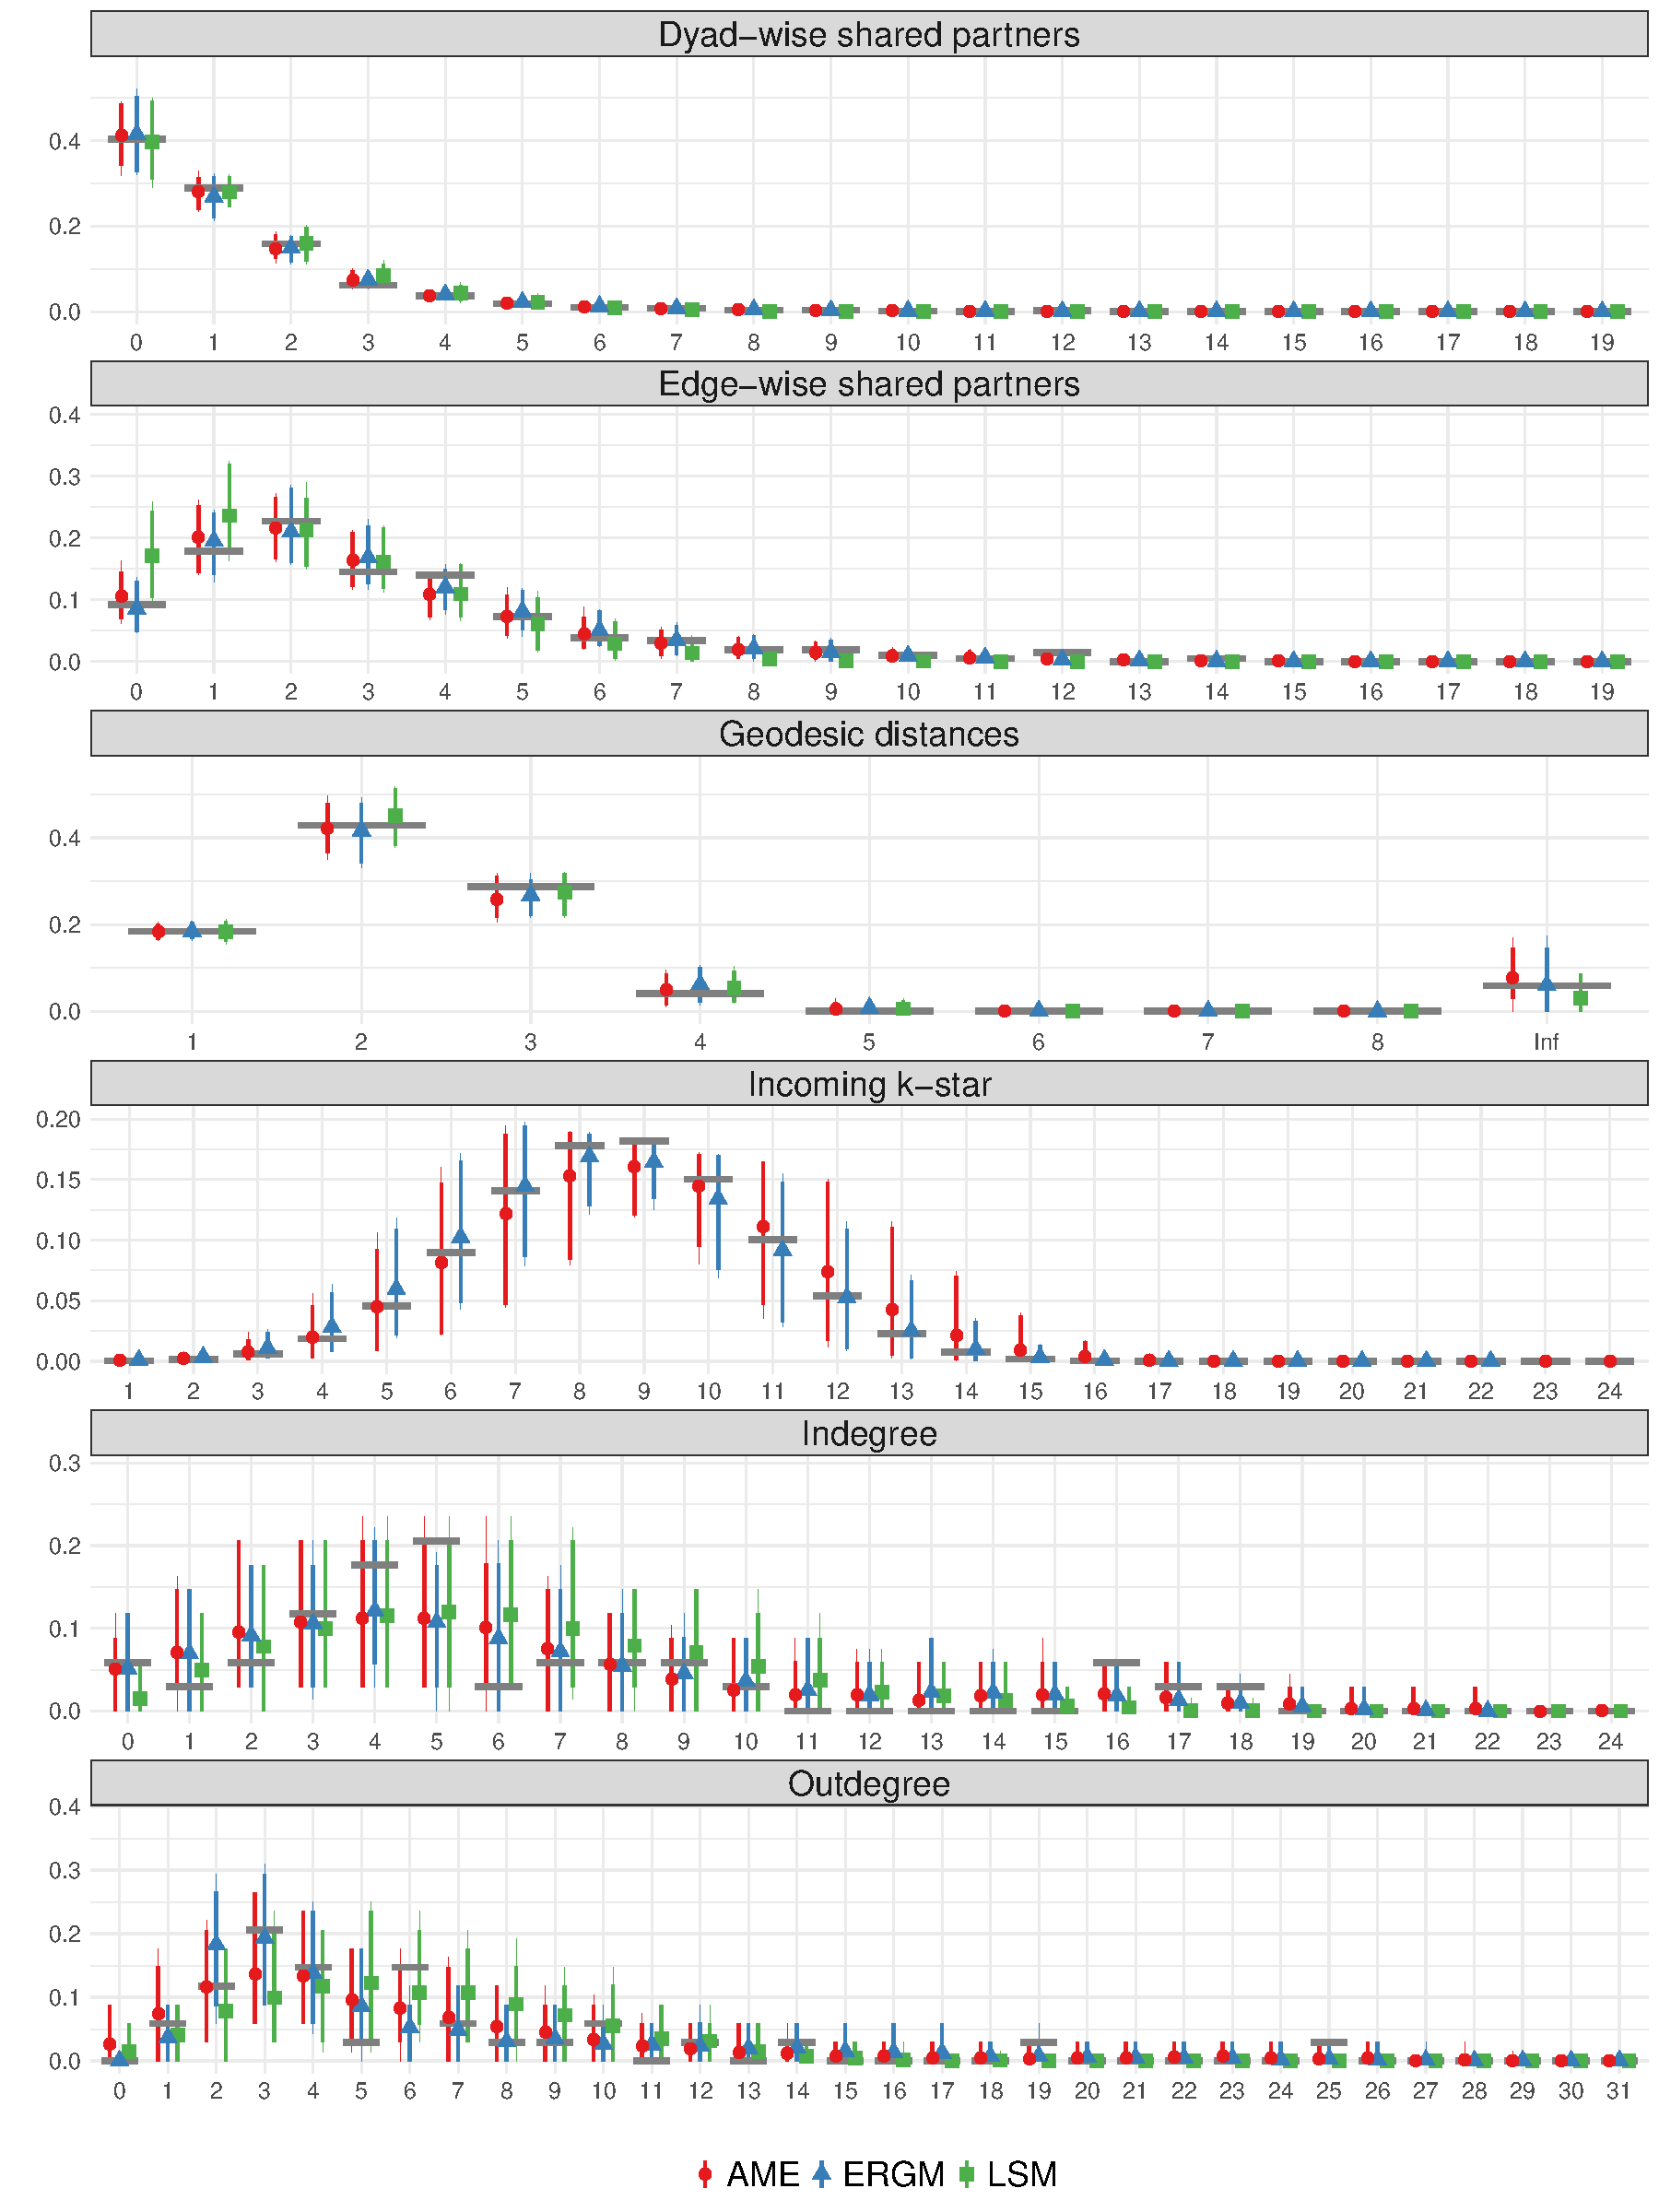
\includegraphics[width=1\textwidth]{ggGofAll}
	\caption{network stats }
	\label{fig:gofAll}
\end{figure}

Figure~\ref{fig:ergmAmePerf} give posterior predictive goodness of fit summaries for four network statistics: (1) the empirical standard deviation of the row means; (2) the empirical standard deviation of the column means (heterogeneity of nodes with incoming activity); (3) the empirical within-dyad correlation; (4) a normalized measure of triadic dependence \citep{hoff:etal:2015}. 

For a given summary statistic g() we first simulate $\mathbf{Y}_{sim} \approx p(\mathbf{Y}_{sim} | \mathbf{Y}_{obs}) = \int p(\mathbf{Y}_{sim} | \theta) p(d \theta | \mathbf{Y}_{obs})$ and then we compare $g(\mathbf{Y}_{sim})$ to $g(\mathbf{Y}_{obs})$. Histograms represent predicted value of statistics under the model and red dash line represents the observed value. 

Proportion of ties that are reciprocated. 

\begin{align}
\begin{aligned}
t(Y) &= \frac{ \sum_{i \neq j}y_{i,j} y_{j,i} }{ \sum_{i \neq j} y_{i,j} } \\
\end{aligned}
\end{align}

Number of transitive triplets, number of triangles in network, number of times ijk are all connected.

\begin{align}
\begin{aligned}
t(Y) &= \sum_{i \neq j \neq k} y_{i,j} y_{i,k} y_{j,k}
\end{aligned}
\end{align}

\begin{figure}[ht]
	\centering
	\includegraphics[width=1\textwidth]{netPerfCoef}
	\caption{Posterior predictive goodness of fit summary}
	\label{fig:ergmAmePerf}
\end{figure}
\FloatBarrier
\section{\textbf{Conclusion}}

The AME approach that we introduce here is a flexible scheme that can be used to handle relational data structures arising from a variety of distributions and is also able to estimate models on longitudinal relational data structures. As we have noted throughout this paper relational data structures are composed of actors that are part of a system, it is highly unlikely that this system can be viewed simply as a collection of isolated dyads. The assumption should be that dependencies between observations likely exist and at the very least we should test for them. Failure to take into account interdependencies leads to biased parameter estimates and a model that will likely be a very poor fit to the data. Further through using diagnostics such as the ones we discussed in Figures~\ref{fig:gofAll} and \ref{fig:ergmAmePerf}, one can easily assess whether an assumption of independence is reasonable and from there decide on the simplest approach to proceed.


\clearpage

\renewcommand{\thefigure}{A\arabic{figure}}
\setcounter{figure}{0}
\renewcommand{\thetable}{A.\arabic{table}}
\setcounter{table}{0}
\renewcommand{\thesection}{A.\arabic{section}}
\setcounter{section}{0}

\section{\textbf{Appendix}}

\subsection{AME Model Convergence}
\label{sec:ameConvAppendix}

Trace plot for AME model presented in paper.  

\begin{figure}[ht]
	\centering
	\begin{tabular}{cc}
	\includegraphics[width=.45\textwidth]{ameConv1_SR2} &
	\includegraphics[width=.45\textwidth]{ameConv2_SR2}
	\end{tabular}
	\caption{Trace plot for AME model presented in paper. In this model, we utilize the SRM to account for first and second-order dependence. To account for third order dependencies we use the latent factor approach with $K=2$.}
	\label{fig:ameConv}
\end{figure}
\FloatBarrier
\newpage

\subsection{Comparison of \pkg{amen} \& \pkg{latentnet} $\mathcal{R}$ Packages}
\label{sec:ameVsLatentnetAppendix}

Here we provide a comparison of the AME model we present in the paper with a variety of parameterizations from the \pkg{latentnet} package. The number of dimensions in the latent space in each of these cases is set to 2. LSM (SR) represents a model in which random sender and receiver effects are included. LSM (Bilinear) represents a model in which a bilinear latent model term is used instead of the default Euclidean distance term. A bilinear latent model with sender and receiver random effects is not equivalent to the AME approach that we introduce here for reasons that we have already discussed in the paper. 

% latex table generated in R 3.3.1 by xtable 1.8-2 package
% Sun Aug 21 03:38:39 2016
\begin{table}[ht]
\centering
\begingroup\tiny
\begin{tabular}{lccccc}
   & LSM & LSM (Bilinear) & LSM (SR) & LSM (Bilinear + SR) & AME \\ 
  \hline
\hline
Intercept/Edges & 0.94$^{\ast}$ & -2.66$^{\ast}$ & 0.60 & -2.50$^{\ast}$ & -3.39$^{\ast}$ \\ 
   & [0.09; 1.82] & [-3.53; -1.87] & [-1.10; 2.37] & [-4.14; -0.88] & [-4.38; -2.50] \\ 
  \textbf{Conflicting policy preferences} &  &  &  &  &  \\ 
  $\;\;\;\;$ Business vs. NGO & -1.37$^{\ast}$ & -2.64$^{\ast}$ & -3.07$^{\ast}$ & -2.87$^{\ast}$ & -1.37$^{\ast}$ \\ 
   & [-2.42; -0.41] & [-4.61; -0.96] & [-4.77; -1.56] & [-4.63; -1.29] & [-2.44; -0.47] \\ 
  $\;\;\;\;$ Opposition/alliance & 0.00 & 0.04 & 0.31 & 0.24 & 1.08$^{\ast}$ \\ 
   & [-0.40; 0.39] & [-0.44; 0.54] & [-0.24; 0.86] & [-0.36; 0.82] & [0.72; 1.47] \\ 
  $\;\;\;\;$ Preference dissimilarity & -1.76$^{\ast}$ & -2.00$^{\ast}$ & -1.88$^{\ast}$ & -2.20$^{\ast}$ & -0.79$^{\ast}$ \\ 
   & [-2.62; -0.90] & [-3.01; -1.03] & [-3.07; -0.68] & [-3.46; -0.96] & [-1.55; -0.08] \\ 
  \textbf{Transaction costs} &  &  &  &  &  \\ 
  $\;\;\;\;$ Joint forum participation & 1.51$^{\ast}$ & 1.24$^{\ast}$ & 1.56$^{\ast}$ & 1.62$^{\ast}$ & 0.92$^{\ast}$ \\ 
   & [0.86; 2.17] & [0.53; 1.93] & [0.69; 2.41] & [0.70; 2.52] & [0.40; 1.47] \\ 
  \textbf{Influence} &  &  &  &  &  \\ 
  $\;\;\;\;$ Influence attribution & 0.08 & -0.08 & 0.30 & 0.28 & 1.09$^{\ast}$ \\ 
   & [-0.40; 0.55] & [-0.62; 0.46] & [-0.37; 0.96] & [-0.42; 0.97] & [0.69; 1.53] \\ 
  $\;\;\;\;$ Alter's influence indegree & 0.01 & -0.05$^{\ast}$ & 0.06 & 0.05 & 0.11$^{\ast}$ \\ 
   & [-0.03; 0.04] & [-0.09; -0.01] & [-0.03; 0.14] & [-0.04; 0.13] & [0.07; 0.15] \\ 
  $\;\;\;\;$ Influence absolute diff. & 0.04 & 0.02 & -0.08$^{\ast}$ & -0.08$^{\ast}$ & -0.07$^{\ast}$ \\ 
   & [-0.01; 0.09] & [-0.03; 0.07] & [-0.14; -0.02] & [-0.14; -0.02] & [-0.11; -0.03] \\ 
  $\;\;\;\;$ Alter = Government actor & -0.46 & -0.80 & -0.11 & -0.20 & 0.55 \\ 
   & [-1.08; 0.14] & [-1.67; 0.04] & [-1.91; 1.76] & [-2.14; 1.74] & [-0.07; 1.15] \\ 
  \textbf{Functional requirements} &  &  &  &  &  \\ 
  $\;\;\;\;$ Ego = Environmental NGO & -0.60 & -1.90$^{\ast}$ & -1.69 & -1.84 & 0.67 \\ 
   & [-1.32; 0.09] & [-3.10; -0.86] & [-3.74; 0.23] & [-4.02; 0.11] & [-0.38; 1.71] \\ 
  $\;\;\;\;$ Same actor type & 1.17$^{\ast}$ & 1.40$^{\ast}$ & 1.82$^{\ast}$ & 1.90$^{\ast}$ & 1.04$^{\ast}$ \\ 
   & [0.63; 1.71] & [0.85; 1.95] & [1.10; 2.54] & [1.19; 2.62] & [0.63; 1.50] \\ 
   \hline
\hline
\end{tabular}
\endgroup
\caption{* p $<$ 0.05. 95\% posterior credible intervals are provided in brackets.} 
\label{tab:regTable_latSpace}
\end{table}


\begin{figure}[ht]
	\centering
	\begin{tabular}{cc}
	\includegraphics[width=.5\textwidth]{roc_latSpace_outSample} & 
	\includegraphics[width=.5\textwidth]{rocPr_latSpace_outSample}
	\end{tabular}
	\caption{Assessments of out-of-sample predictive performance using ROC curves, separation plots, and PR curves. AUC statistics are provided as well for both curves.}
	\label{fig:roc_latentSpace}
\end{figure}

\begin{figure}[ht]
	\centering
	\includegraphics[width=1\textwidth]{netPerfCoef_latSpace}
	\caption{Network goodness of fit summary using \pkg{amen}.}
	\label{fig:netPerfCoef_latSpace}
\end{figure}

% \begin{figure}[ht]
% 	\centering
% 	\includegraphics[width=1\textwidth]{ggGofAll_latSpace}
% 	\caption{network stats }
% 	\label{fig:gofAll_latSpace}
% \end{figure}
\FloatBarrier

\clearpage
\subsection{Comparison with other AME Parameterizations}
\label{sec:ameVsAmeAppendix}

Here we provide a comparison of the AME model we present in the paper that uses $K=2$ for multiplicative effects and show how results change when we use $K=\{1,3,4\}$. Trace plots for $K=\{1,3,4\}$ are available upon request.

% latex table generated in R 3.5.0 by xtable 1.8-2 package
% Wed Jul 11 18:23:00 2018
\begin{table}[ht]
\centering
\begingroup\tiny
\begin{tabular}{lcccc}
   & AME (k=1) & AME (k=2) & AME (k=3) & AME (k=4) \\ 
  \hline
\hline
Intercept/Edges & -3.07 & -3.40 & -3.91 & -4.13 \\ 
   & [-3.87; -2.29] & [-4.40; -2.51] & [-5.90; -2.82] & [-5.93; -3.00] \\ 
  \textbf{Conflicting policy preferences} &  &  &  &  \\ 
  $\;\;\;\;$ Business vs. NGO & -1.27 & -1.38 & -1.52 & -1.54 \\ 
   & [-2.19; -0.47] & [-2.47; -0.49] & [-2.67; -0.53] & [-2.59; -0.47] \\ 
  $\;\;\;\;$ Opposition/alliance & 0.94 & 1.08 & 1.27 & 1.38 \\ 
   & [0.66; 1.27] & [0.72; 1.49] & [0.82; 2.10] & [0.87; 2.24] \\ 
  $\;\;\;\;$ Preference dissimilarity & -0.65 & -0.79 & -0.90 & -0.94 \\ 
   & [-1.28; -0.04] & [-1.55; -0.07] & [-1.78; -0.13] & [-1.77; -0.08] \\ 
  \textbf{Transaction costs} &  &  &  &  \\ 
  $\;\;\;\;$ Joint forum participation & 0.84 & 0.92 & 1.08 & 1.22 \\ 
   & [0.38; 1.31] & [0.40; 1.46] & [0.41; 1.96] & [0.50; 2.24] \\ 
  \textbf{Influence} &  &  &  &  \\ 
  $\;\;\;\;$ Influence attribution & 1.00 & 1.10 & 1.30 & 1.39 \\ 
   & [0.65; 1.40] & [0.70; 1.55] & [0.76; 2.29] & [0.82; 2.27] \\ 
  $\;\;\;\;$ Alter's influence indegree & 0.10 & 0.11 & 0.13 & 0.14 \\ 
   & [0.07; 0.13] & [0.07; 0.15] & [0.09; 0.20] & [0.09; 0.21] \\ 
  $\;\;\;\;$ Influence absolute diff. & -0.06 & -0.07 & -0.08 & -0.09 \\ 
   & [-0.09; -0.03] & [-0.11; -0.03] & [-0.15; -0.04] & [-0.16; -0.04] \\ 
  $\;\;\;\;$ Alter = Government actor & 0.52 & 0.56 & 0.65 & 0.72 \\ 
   & [0.00; 1.08] & [-0.06; 1.16] & [-0.05; 1.49] & [-0.01; 1.48] \\ 
  \textbf{Functional requirements} &  &  &  &  \\ 
  $\;\;\;\;$ Ego = Environmental NGO & 0.62 & 0.68 & 0.84 & 0.86 \\ 
   & [-0.28; 1.53] & [-0.36; 1.73] & [-0.43; 2.40] & [-0.49; 2.32] \\ 
  $\;\;\;\;$ Same actor type & 0.98 & 1.03 & 1.17 & 1.23 \\ 
   & [0.60; 1.37] & [0.62; 1.48] & [0.69; 1.83] & [0.70; 1.96] \\ 
   \hline
\hline
\end{tabular}
\endgroup
\caption{* p $<$ 0.05 (or 0 outside the 95\% confidence interval).} 
\label{tab:regTable_latSpace}
\end{table}


\begin{figure}[ht]
	\centering
	\begin{tabular}{cc}
	\includegraphics[width=.5\textwidth]{roc_ameSR_outSample} & 
	\includegraphics[width=.5\textwidth]{rocPr_ameSR_outSample}
	\end{tabular}
	\caption{Assessments of out-of-sample predictive performance using ROC curves, separation plots, and PR curves. AUC statistics are provided as well for both curves.}
	\label{fig:roc_ame}
\end{figure}

\begin{figure}[ht]
	\centering
	\includegraphics[width=1\textwidth]{netPerfCoef_ameSR}
	\caption{Network goodness of fit summary using \pkg{amen}.}
	\label{fig:netPerfCoef_ameSR}
\end{figure}

% \begin{figure}[ht]
% 	\centering
% 	\includegraphics[width=1\textwidth]{ggGofAll_ameSR}
% 	\caption{network stats }
% 	\label{fig:gofAll_ameSR}
% \end{figure}
\FloatBarrier

% \newpage
% \begin{figure}[ht]
% 	\centering
% 	\begin{tabular}{cc}
% 	\includegraphics[width=.45\textwidth]{ameConv1_SR1} &
% 	\includegraphics[width=.45\textwidth]{ameConv2_SR1}
% 	\end{tabular}
% 	\caption{Trace plot for AME model in which we utilize the SRM to account for first and second-order dependence. To account for third order dependencies we use the latent factor approach with $K=1$.}
% 	\label{fig:ameConv}
% \end{figure}

% \begin{figure}[ht]
% 	\centering
% 	\begin{tabular}{cc}
% 	\includegraphics[width=.45\textwidth]{ameConv1_SR3} &
% 	\includegraphics[width=.45\textwidth]{ameConv2_SR3}
% 	\end{tabular}
% 	\caption{Trace plot for AME model in which we utilize the SRM to account for first and second-order dependence. To account for third order dependencies we use the latent factor approach with $K=3$.}
% 	\label{fig:ameConv}
% \end{figure}
% \FloatBarrier

% \begin{figure}[ht]
% 	\centering
% 	\begin{tabular}{cc}
% 	\includegraphics[width=.45\textwidth]{ameConv1_SR4} &
% 	\includegraphics[width=.45\textwidth]{ameConv2_SR4}
% 	\end{tabular}
% 	\caption{Trace plot for AME model in which we utilize the SRM to account for first and second-order dependence. To account for third order dependencies we use the latent factor approach with $K=4$.}
% 	\label{fig:ameConv}
% \end{figure}


\newpage

% Bib stuff
\clearpage
\bibliography{{/Users/janus829/whistle/master}, {/Users/s7m/whistle/master}, {/Users/mdw/git/whistle/master}}
% \bibliography{/Users/mdw/git/whistle/master}
\bibliographystyle{elsarticle-harv}\biboptions{authoryear}
\newpage

\end{document} 